\section{Анализ предметной области}

На данном этапе работы будет обоснована актуальность темы. Также необходимо рассмотреть основные области, которые затрагивает разрабатываемая система. Сюда входят такие темы, как методы сбора данных, а также методы их анализа и обработки. Кроме того, нужно описать, почему важна персонализация услуг и предложений, на основе интересов клиентов.

\subsection{Актуальность темы}

Сбор и анализ данных о предпочтениях владельцев автомобилей представляет собой важный аспект для улучшения качества обслуживания и удовлетворения их потребностей. Традиционные методы исследований, такие как опросы и анкетирование, часто требуют значительных усилий и временных затрат для обработки и анализа полученных данных. Однако, использование современных методов машинного обучения и анализа данных открывает новые возможности для автоматизации этого процесса.

Данный проект направлен на создание модуля, способного автоматически анализировать предпочтения владельцев автомобилей на основе данных о модели автомобиля и возрасте. Этот подход позволяет существенно сократить время, затрачиваемое на сбор и обработку данных, а также предоставляет более точную и полную информацию о предпочтениях владельцев.

В условиях растущей конкуренции в автомобильной индустрии, эффективное использование данных о предпочтениях клиентов становится ключевым конкурентным преимуществом. Автоматизированный анализ интересов владельцев автомобилей позволит нам лучше понять их потребности, оптимизировать наши услуги и предложения, и разработать персонализированные подходы для каждого клиента.

Ключевым аспектом проекта является определение наиболее подходящих методов сбора данных. Это включает в себя исследование различных источников информации, таких как базы данных регистраций автомобилей, данные из социальных сетей, онлайн-опросы и другие методы. Важно выбрать те методы, которые обеспечат наибольшую точность и актуальность получаемых данных, а также будут соответствовать требованиям конфиденциальности и защиты информации.

После сбора данных необходимо обеспечить их качественную обработку и анализ. Это включает очистку данных, устранение пропусков и ошибок, а также применение методов машинного обучения и аналитических инструментов для выявления закономерностей и трендов. Важным аспектом является также визуализация данных, которая позволит легко интерпретировать результаты анализа и принимать обоснованные решения на их основе.

Таким образом, разработка модуля для анализа предпочтений владельцев автомобилей на основе современных методов машинного обучения представляет собой актуальное и перспективное направление в области обслуживания клиентов.




\subsection{Методы сбора данных}

% Сбор данных представляет собой процесс измерения и накопления информации о необходимых 
% переменных, что позволяет задавать и решать различные исследовательские вопросы. Этот процесс 
% является неотъемлемой частью обучения в таких дисциплинах, как маркетинг, статистика, 
% экономика, естественные науки и других. Методы сбора информации могут отличаться в зависимости от 
% специфики предмета, однако цель исследования и добросовестность в данном процессе остаются 
% одинаково важными во всех областях знаний. Сбор данных играет ключевую роль, 
% поскольку он позволяет принимать обоснованные и систематические решения. Данные представляют 
% собой незаменимый инструмент для принятия взвешенных решений, экономя как время, так и ресурсы. 

Сбор данных является процессом, включающим измерение и накопление информации о важных переменных, что позволяет формулировать и решать различные исследовательские вопросы. Этот процесс занимает ключевое место в образовательных программах по маркетингу, статистике, экономике, естественным наукам и другим дисциплинам. Методы сбора информации могут варьироваться в зависимости от особенностей предмета, однако цель исследования и добросовестность в этом процессе остаются одинаково значимыми во всех областях знаний. Сбор данных имеет решающее значение, так как позволяет принимать обоснованные и систематические решения. Данные служат незаменимым инструментом для принятия обдуманных решений, экономя время и ресурсы \refref{ref:data-collection}.

В зависимости от характера сбора данных их можно разделить на два основных типа, а именно \refref{ref:data-collection}:

\begin{itemize}
	\item первичный метод;
	\item вторичный метод.
\end{itemize}

Первичные данные исследователи получают самостоятельно и впервые в контексте своего исследования.
Существуют несколько способов сбора первичных данных \refref{ref:data-collection}:

\begin{itemize}
	\item интервью. Интервью являются наиболее распространенным методом первичного сбора данных. В ходе интервью исследователь использует анкету или задает вопросы непосредственно респонденту. Основная цель состоит в том, чтобы получить информацию по интересующим темам из ответов участников. Анкеты могут быть отправлены по электронной почте, либо детали могут быть уточнены в ходе телефонного интервью;
	\item метод Дельфи. В этом методе исследователь обращается за информацией к группе экспертов. Он может провести исследование очно или отправить анкеты по электронной почте. По завершении применения метода Дельфи все данные собираются и обрабатываются в соответствии с потребностями исследования;
	\item проективные методы. Проективные методы применяются в исследованиях, где вопросы касаются частной или конфиденциальной информации, и исследователь полагает, что респонденты не раскроют данные при прямом опросе. Существует множество типов проективных методик, таких как тематические апперцептивные тесты, ролевые игры, завершение мультфильмов, словесные ассоциации и завершение предложений;
	\item интервью в фокус-группе. Для обсуждения насущной проблемы собирается группа из нескольких человек. В таких интервью обычно участвует от шести до двенадцати человек. Каждый участник высказывает свое мнение, и в итоге принимается коллективное единогласное решение;
	\item метод анкетирования. Здесь используется вопросник для сбора данных от различных 
	групп населения. Для сбора данных от различных групп населения используется вопросник. В соответствующем исследовании применяется набор вопросов, на которые респонденты отвечают, прямо или косвенно связанные с темой вопросника.
\end{itemize}

Эти методы позволяют анализировать большие объемы информации и выявлять статистически значимые закономерности, что способствует более обоснованным выводам и рекомендациям.

Вторичные данные означают данные, которые исследователь собирает не самостоятельно и в 
раз. Фактически, вторичные данные уже доступны и их необходимо собирать из различных 
источников \refref{ref:data-collection}.

Некоторые источники данных, которые могут быть использованы для вторичного сбора данных, 
включают \refref{ref:data-collection}:

\begin{itemize}
	\item газеты;
	\item журналы;
	\item публичные записи;
	\item деловые документы;
	\item исторические и статистические документы и т.д.
\end{itemize}

Помимо упомянутых выше опубликованных источников данных, для вторичного сбора информации могут использоваться неопубликованные данные, такие как письма, дневники и неопубликованные биографии \refref{ref:data-collection}.

Количественные методы первичного сбора данных могут быть различных типов, некоторые из 
которых следующие \refref{ref:data-collection}:

\begin{itemize}
	\item вероятностная выборка. В этом методе в целевой совокупности используется форма случайного отбора. Затем на основе данных, полученных от случайной выборки, делаются вероятностные утверждения о генеральной совокупности. Преимущество случайной выборки заключается в том, что исследователи могут собирать данные от представителей, а не от всей популяции, что позволяет получить в основном беспристрастные данные;
	\item интервью. Интервью также являются отличным способом сбора первичных данных. Собеседования могут проводиться тремя способами: по телефону, очно и с использованием компьютера. Цель интервью состоит в быстром и эффективном получении объективных персональных данных о респондентах;
	\item опросы. Анкетирование также представляет собой отличный метод сбора первичных данных. Анкеты могут быть распространены по электронной почте или через интернет. Основная цель опросов - быстрое получение данных в форме, которую легко проверить. Это также очень простой способ собрать первичные данные от населения;
	\item наблюдения. Наблюдения также представляют собой очень простой способ сбора количественных данных. В процессе наблюдения за группой населения в определенной демографической зоне собираются данные, связанные с первичным исследованием. 
\end{itemize}

Теперь поговорим про методы сбора качественных данных.
Многие методы сбора данных могут быть использованы как для сбора количественной, так и для сбора качественной информации. Интервью, например, могут быть структурированными, чтобы собирать количественные данные, или полуструктурированными или неструктурированными, чтобы собирать более глубокие качественные данные. То же самое относится и к наблюдениям: они могут быть использованы для сбора как количественных, так и качественных данных в зависимости от методологии и целей исследования \refref{ref:data-collection}.

Опросы, групповые обсуждения, наблюдения и интервью являются часто используемыми методами сбора качественных данных. Кроме того, такие методы, как методика Дельфи и проективные методики, также могут быть использованы для сбора качественных данных в зависимости от специфики исследования и целей исследователя.

Качественные данные, часто представленные в виде текстовой информации, играют важную роль в исследованиях и анализе. Поддержание допустимой погрешности в качественных данных существенно для получения достоверной картины результатов исследования. В то же время количественные данные должны быть максимально точными, поскольку они непосредственно влияют на результаты исследования. Такое разделение помогает исследователям адекватно оценивать и интерпретировать данные в соответствии с целями и характером исследования \refref{ref:data-collection}.


\subsection{Обработка и анализ данных}

Обработка и анализ данных - это критически важный этап, включающий преобразование и толкование информации с целью выявления закономерностей, паттернов и тенденций. С увеличением объема и разнообразия данных в современном мире становится необходимым использование разнообразных методов и инструментов для их полноценного анализа. Это включает в себя как классические статистические методы, так и современные техники машинного обучения и анализа больших данных. Грамотный анализ данных позволяет выявить скрытые закономерности и важные тренды, что в свою очередь помогает принимать обоснованные решения и формулировать стратегии на основе фактических данных \refref{ref:data-analysis}.

\subsubsection{Методы предобработки данных}

Предобработка данных играет важную роль в процессе обработки информации, нацеленной на подготовку данных для дальнейшего анализа. Она включает в себя процессы, такие как очистка данных от выбросов и ошибок, заполнение пропущенных значений, масштабирование признаков и преобразование категориальных признаков в числовые. Эти шаги направлены на создание более чистого и пригодного для анализа набора данных, что способствует более точному и надежному анализу и интерпретации результатов \refref{ref:data-analysis}.

Предварительная обработка данных включает выполнение следующих этапов \refref{ref:data-analysis}:

\begin{enumerate}
	\item проверка целостности данных;
	\item очистка данных от ошибок и аномалий;
	\item преобразование данных в удобный формат;
	\item добавление новых данных для повышения информативности;
	\item улучшение эффективности обработки данных.
\end{enumerate}

Проверка данных включает в себя обнаружение \refref{ref:data-analysis}:

\begin{itemize}
	\item дублирующихся записей, несоответствий и ошибок;
	\item необычных или аномальных наблюдений;
	\item пропущенных значений.
\end{itemize}

Очистка данных включает \refref{ref:data-analysis}:

\begin{itemize}
	\item удаление повторяющихся записей, несоответствий и ошибок;
	\item обработку необычных или аномальных наблюдений;
	\item заполнение пропущенных значений.
\end{itemize}

При работе с данными важно правильно обрабатывать пропущенные значения. Этот процесс является важным этапом работы с данными. Удаление пропусков может быть необходимым, но такой подход требует внимательного анализа и оценки влияния на результаты исследования. В некоторых случаях удаление может привести к искажению данных или потере важной информации. Пропускание пропущенных значений - еще один способ обработки, который может быть применен, если пропуски не существенно влияют на анализ. Заполнение пропущенных значений - еще одна распространенная стратегия, которая позволяет сохранить данные и избежать искажений. Все эти методы требуют осторожности и обоснованного подхода в зависимости от конкретной ситуации и характера данных.
Пропущенные значения можно заполнить \refref{ref:data-analysis}:

\begin{itemize}
	\item нулевыми значениями;
	\item модой, медианой или средним значением;
	\item использованием индикаторных переменных.
\end{itemize}

Преобразование данных включает в себя \refref{ref:data-analysis}:

\begin{itemize}
	\item изменение названий признаков;
	\item сортировку и группировку данных;
	\item кодирование переменных;
	\item нормализацию данных.
\end{itemize}

Добавление данных предполагает создание новых признаков и объединение существующих.
Улучшение эффективности обработки данных включает \refref{ref:data-analysis}:

\begin{itemize}
	\item сокращение размерности;
	\item идентификацию и исключение незначительных признаков.
\end{itemize}

\subsubsection{Методы визуализации данных}

Визуализация данных играет ключевую роль в исследовании и анализе данных, помогая выявить визуальные закономерности и тренды. Она позволяет представить данные в понятной и наглядной форме с использованием различных графических элементов, таких как графики, диаграммы, и карты. Визуализация делает данные более доступными для понимания и интерпретации как для специалистов, так и для широкой аудитории. Этот инструмент позволяет исследователям и аналитикам обнаруживать важные закономерности и взаимосвязи в данных, что в свою очередь помогает принимать обоснованные решения и формулировать стратегии на основе данных \refref{ref:data-visualization}.

Существует несколько видов визуализации \refref{ref:data-visualization}:

\begin{itemize}
	\item обычные графические представления. Он включает в себя различные виды диаграмм и графиков, используемых для отображения количественной информации. Круговые диаграммы, например, используются для представления долей целого, линейные диаграммы отображают изменение величин с течением времени, гистограммы представляют распределение данных по интервалам, а точечные графики позволяют визуализировать взаимосвязи между двумя переменными. Эти стандартные методы визуализации являются основой для анализа данных и широко используются в научных и бизнес-исследованиях для визуального представления количественной информации;
	\item преобразование данных. Он позволяет изменить формат данных для более наглядного восприятия. Например, карты используются для визуализации пространственных данных, а полярные графики отображают данные в полярной координатной системе. Также сюда относятся временные линии, которые представляют изменение данных во времени, и графики с параллельными осями, используемые для сравнения нескольких категорий данных. Эти методы визуализации помогают улучшить понимание данных и выявить закономерности, которые могут быть невидимы при простом представлении данных;
	\item концептуальная визуализация. Она используется для представления сложных концепций, идей и планов. К этому типу визуализации относятся концептуальные карты, которые помогают организовать и визуализировать связанные идеи, и диаграммы Ганта, используемые для планирования и отслеживания проектов с учетом временных рамок. Эти инструменты помогают упростить восприятие и понимание сложных идей и процессов, делая их более доступными для анализа и интерпретации;
	\item стратегическая визуализация. Этот тип визуализации включает в себя различные диаграммы, такие как графики жизненного цикла продукта, которые отображают этапы развития продукта, и структурные графики организаций, показывающие их иерархию и взаимосвязи. Эти инструменты помогают руководителям и аналитикам лучше понимать внутренние процессы, оценивать эффективность и разрабатывать стратегические планы;
	\item метафорическая визуализация. Это способ представления данных с помощью метафор, чтобы сделать их более понятными. Например, карта метро может показать, как разные категории информации связаны друг с другом, а пирамиды или деревья могут продемонстрировать иерархические структуры. Этот подход помогает легче воспринимать сложные данные, используя знакомые образы;
	\item комбинированная визуализация. Этот тип визуализации объединяет разные виды графиков и диаграмм в одном изображении, чтобы более полно представить данные. Например, карта прогноза погоды может показывать одновременно температуру, осадки и ветер. Такой способ помогает лучше понять данные, поскольку вся информация представлена вместе и легко доступна для анализа.
\end{itemize}

Визуализация помогает быстрее и эффективнее донести результаты анализа до заинтересованных сторон, улучшая понимание и принятие решений.

\subsubsection{Методы машинного обучения}

Корни технологии машинного обучения, основанной на анализе данных, уходят еще в 1950-е годы, когда появились первые программы для игры в шашки. С течением времени, при сохранении общего принципа, эта область претерпела значительные изменения благодаря росту вычислительной мощности компьютеров. Это привело к усложнению методов анализа данных и прогнозирования, а также к расширению спектра задач, которые можно решить с использованием машинного обучения \refref{ref:machine-learning}.

Процесс машинного обучения начинается с загрузки исходных данных, известных как датасет. Например, это могут быть помеченные фотографии собак и кошек. После обучения на этих данных алгоритм способен распознавать собак и кошек на новых изображениях без пометок. Процесс обучения не заканчивается после первых прогнозов: чем больше данных анализируется, тем выше точность модели в распознавании нужных изображений \refref{ref:machine-learning}.

Машинное обучение позволяет компьютерам не только распознавать лица на фотографиях, но и анализировать пейзажи, объекты, текст и цифры. Для анализа текста также используются методы машинного обучения. Функция проверки грамматики, доступная во многих текстовых редакторах и мобильных приложениях, учитывает не только правильность написания слов, но и контекст, смысловые оттенки и другие лингвистические аспекты. Кроме того, существует программное обеспечение, способное автоматически создавать новостные статьи (например, о событиях в экономике и спорте) без участия человека \refref{ref:machine-learning}.

Типы задач машинного обучения \refref{ref:machine-learning}:

\begin{itemize}
	\item задача регрессии. Суть заключается в предсказании числового значения на основе определенного набора признаков. Например, это может быть прогноз цены квартиры на основе таких факторов, как площадь, количество комнат, расположение и другие характеристики. Также задача регрессии может применяться для предсказания ожидаемого дохода магазина на основе таких факторов, как расположение, количество посетителей, временной период и прочее. Основная цель регрессионного анализа - построить модель, которая бы максимально точно предсказывала зависимую переменную на основе доступных признаков;
	\item задача классификации. Суть заключается в присвоении объекту одной из категорий на основе его признаков. Например, это может быть определение, есть ли на фотографии кошка или собака, или является ли письмо спамом или не спамом. Для решения задачи классификации используются алгоритмы машинного обучения, которые обучаются на размеченных данных и способны классифицировать новые объекты на основе изученных характеристик. Основная цель классификационного анализа - построить модель, которая бы максимально точно разделяла объекты на заданные классы;
	\item задача кластеризации. Суть заключается в разделении данных на группы или кластеры на основе их сходства. Например, в контексте разделения клиентов по уровню платежеспособности, алгоритм кластеризации может автоматически выделить группы клиентов с похожими характеристиками или поведением в отношении платежей. Это позволяет более эффективно анализировать и работать с данными, выявляя закономерности и тренды внутри каждой группы;
	\item задача уменьшения размерности. Суть заключается в сокращении количества признаков в данных с сохранением максимально возможной информации. Например, это может быть сжатие данных для удобства визуализации на графиках. При использовании методов уменьшения размерности данные проецируются из исходного пространства высокой размерности в пространство меньшей размерности, при этом стараясь сохранить как можно больше вариативности и структуры данных. Это позволяет сократить количество признаков для анализа данных, уменьшить их размер и облегчить визуализацию без значительной потери информации;
	\item задача выявления аномалий. Суть заключается в обнаружении нестандартных или нетипичных случаев среди данных. Например, это может быть выявление мошеннических операций с банковскими картами среди обычных финансовых транзакций. Для решения этой задачи используются методы машинного обучения, которые строят модели на основе нормального поведения данных и выявляют аномалии как объекты, сильно отклоняющиеся от этого нормального шаблона. Выявление аномалий имеет важное значение в областях безопасности, финансов, здравоохранения и других, где даже небольшие отклонения могут иметь серьезные последствия.
\end{itemize}

Методы машинного обучения можно разделить на два основных класса: обучение с учителем и обучение без учителя \refref{ref:machine-learning}.

В случае обучения с учителем модели предоставляются правильные ответы для обучающих данных. Эти данные состоят из пар "входные признаки - правильные ответы". Модель обучается на таких данных с целью научиться предсказывать правильные ответы для новых, ранее не виданных данных \refref{ref:machine-learning}.

В случае обучения без учителя модели не предоставляются правильные ответы. Модель обучается только на основе входных данных, без информации о правильных ответах. Задача модели здесь состоит в том, чтобы самостоятельно выявить закономерности в данных, например, кластеризовать их или находить структуры и шаблоны, которые могут быть полезны для дальнейшего анализа или решения задач \refref{ref:machine-learning}.

Основные алгоритмы моделей машинного обучения \refref{ref:machine-learning}:

\begin{enumerate}
	\item дерево принятия решений. Дерево принятия решений -  это инструмент, который помогает систематизировать процесс принятия решений. В его основе лежит древовидная структура, где каждый узел представляет собой вопрос, а каждая ветвь - возможный ответ на этот вопрос. Этот метод особенно полезен в бизнесе, где решения часто принимаются на основе конкретных критериев и оценки потенциальных последствий. Пройдя через последовательность вопросов и ответов, можно прийти к логически обоснованному решению;
	\item наивная байесовская классификация. Наивная байесовская классификация - это метод, который используется для разделения данных на категории, основываясь на теореме Байеса и предполагая, что признаки независимы друг от друга. Он применяется в различных областях, включая фильтрацию спама, автоматическую категоризацию текстов, анализ эмоциональной окраски текста, а также в распознавании объектов и лиц на изображениях. Основная идея заключается в том, что каждый признак вносит свой вклад в классификацию независимо от других признаков, делая метод простым и эффективным в некоторых случаях;
	\item метод наименьших квадратов. Метод наименьших квадратов - это способ, используемый в линейной регрессии, чтобы найти прямую, которая наилучшим образом соответствует набору данных. Он основан на минимизации суммы квадратов расстояний от каждой точки данных до этой прямой. В контексте машинного обучения, этот метод помогает уменьшить ошибку при аппроксимации данных и настройке моделей под имеющиеся данные;
	\item логистическая регрессия. Логистическая регрессия - это метод анализа, который используется для определения связи между независимыми переменными и категориальной зависимой переменной. В отличие от линейной регрессии, где зависимая переменная является непрерывной, в логистической регрессии зависимая переменная обычно представляет собой бинарную или категориальную переменную. Этот метод широко применяется в различных областях, таких как кредитный скоринг, анализ результатов маркетинговых кампаний, прогнозирование успешности продуктов и других событий. Он помогает предсказывать вероятность наступления определенного события на основе значений независимых переменных;
	\item метод опорных векторов (SVM). Метод опорных векторов - это набор алгоритмов машинного обучения, который используется для классификации и регрессионного анализа данных. Он работает путем построения гиперплоскости в многомерном пространстве, которая наилучшим образом разделяет точки между двумя классами. SVM пытается максимизировать расстояние между этой гиперплоскостью и ближайшими точками обучающего набора, называемыми опорными векторами.
	\item метод ансамблей. Метод ансамблей в машинном обучении основан на идее создания нескольких классификаторов, которые затем объединяются для принятия решения. Этот подход позволяет уменьшить случайные ошибки и дисперсию модели, а также избежать выхода за пределы предполагаемых гипотез. Изначально метод представлял собой байесовское усреднение, но с течением времени стал более сложным благодаря использованию различных алгоритмов. Он может использовать разнообразные техники, такие как бэггинг, случайный лес, градиентный бустинг и другие, чтобы повысить качество прогнозов;
	\item алгоритмы кластеризации. Кластеризация - это метод, позволяющий объединить объекты в группы таким образом, чтобы объекты внутри одной группы были максимально похожи друг на друга. Алгоритмы кластеризации находят применение в различных областях, включая биологию, социологию и информационные технологии. Например, в биологии они используются для классификации видов или для анализа геномных данных, в социологии - для выявления социальных группировок, а в информационных технологиях - для сегментации пользователей или анализа текстовой информации;
	\item метод главных компонент (PCA). PCA представляет собой статистический метод, который используется для уменьшения размерности данных и визуализации. Он работает путем ортогонального преобразования исходных признаков в новый набор признаков, называемых главными компонентами. Главная цель PCA - сохранить как можно больше информации, содержащейся в исходных данных, при этом снижая количество признаков. Это помогает упростить процесс анализа данных, улучшить производительность моделей машинного обучения и сократить вычислительные затраты;
	\item сингулярное разложение. Сингулярное разложение - это метод линейной алгебры, который разлагает матрицу на три составляющие: левую сингулярную матрицу, правую сингулярную матрицу и диагональную матрицу сингулярных значений. В контексте анализа данных, SVD используется для сжатия данных и уменьшения размерности, что позволяет выделить основные компоненты информации и убрать шумы или ненужные детали, сохраняя при этом основные характеристики данных. Этот метод является основой для таких техник, как метод главных компонент (PCA), и находит широкое применение в различных областях, включая обработку изображений, анализ текстов и рекомендательные системы;
	\item анализ независимых компонент (ICA). Анализ независимых компонент - это метод, который помогает выявить скрытые причины или источники влияния на данные и разделить их на независимые компоненты. Он ищет такие независимые составляющие в наборе данных, которые могут быть полезны для понимания его структуры и свойств. Этот метод особенно полезен в областях, где данные могут быть представлены в виде комбинации различных воздействий или источников.
\end{enumerate}

Методы машинного обучения рассматриваются в проекте для выбора оптимального подхода к анализу данных, что позволяет максимально эффективно и точно решать поставленные задачи. 

\subsubsection{Персонализация услуг и предложений}

В современном мире персонализация услуг и предложений стала краеугольным камнем для бизнеса. Это не просто стратегия, а неотъемлемая часть успешной работы компаний, которая позволяет им лучше понимать и удовлетворять потребности своих клиентов. Главное в этом подходе - создание индивидуального опыта для каждого клиента, учитывая его уникальные характеристики и предпочтения \refref{ref:marketing}.

Конечная цель персонализации - предоставление клиентам наиболее релевантных и ценных продуктов и услуг. Для этого компании активно анализируют данные о своих клиентах, стремясь выявить их индивидуальные потребности и предложить соответствующие решения \refref{ref:marketing}.

Примером может служить использование данных о предпочтениях клиентов для создания персонализированных рекомендаций продуктов или услуг. Если клиент интересуется определенными темами или категориями товаров, компания предлагает ему соответствующие продукты, что может сильно повысить удовлетворенность клиента и вероятность его повторных покупок \refref{ref:marketing}.

В области обслуживания клиентов персонализация также играет решающую роль. Здесь компании стремятся предоставить клиентам индивидуализированный опыт взаимодействия, что включает в себя персонализированные рекомендации, обратную связь и поддержку. Этот подход позволяет укрепить связь с клиентом и повысить его лояльность к бренду \refref{ref:marketing}.

Однако важно помнить, что успешная персонализация невозможна без использования данных для оптимизации маркетинговых усилий и ресурсов компании. Точное нацеливание коммуникации на потребности и интересы клиентов помогает повысить эффективность маркетинговых кампаний и улучшить общее взаимодействие с ними \refref{ref:marketing}.

% \newpage

% \section{Расширенное техническое задание}

% В данном разделе представлено техническое задание на разработку системы.


% \subsection{Основание для разработки}

% Программа разрабатывается на основе учебного плана кафедры “Электронные вычислительные машины” по направлению 09.03.01.

% \subsection{Цель и задача}

% Название темы: «Разработка системы оценки и прогнозирования интересов клиентов автостоянки».

% Целью дипломного проекта является автоматизация процесса сбора данных об интересах посетителей парковки и их прогнозирования.

% Задача – проектирование и разработка системы для сбора информации об интересах и их прогнозирования на базе искусственной нейронной сети.


% \subsection{Наименование и область применения}

% Наименование разрабатываемого программного обеспечения: система оценки и прогнозирования интересов клиентов автостоянки. 

% Область применения: прогнозирование интересов посетителей парковки для улучшения сервиса.


% \subsection{Требования к функциональности}

% Программа должна обеспечивать возможность выполнения следующих функций:

% \begin{itemize}
% 	\item определять регистрационный номер автомобиля;
% 	\item определять модель автомобиля
% 	\item анализировать бланки опросов определенного формата;
% 	\item формирование набора данных в файл типа CSV;
% 	\item обучение нейронной сети по сформированному датасету;
% 	\item предсказывать интересы посетителей с использование обученной модели.
% \end{itemize}


% \subsection{Требования к нейронной сети}

% Нейронная сеть должна быть реализована на базе языка программирования Python с использованием библиотеки Tensorflow, Keras.


% \subsection{Требования к бланку}

% Бланк должен содержать вопросы и варианты ответа на вопросы (ДА/НЕТ), а также поле для ввода возраста. Пример представлен на рисунке~\ref{f:blank}.

% \begin{figure}[ht]
% 	\centering
% 	\vspace{\toppaddingoffigure}
% 	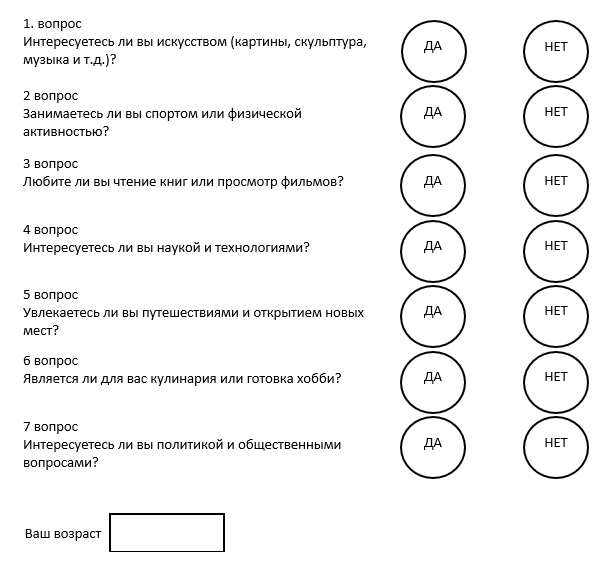
\includegraphics[width=0.7\textwidth]{blank}
% 	\caption{Бланк опроса}
% 	\label{f:blank}
% \end{figure}



% \subsection{Требования к программной документации}

% Состав программной документации должен включать в себя: 

% \begin{itemize}
% 	\item техническое задание; 
% 	\item пояснительная записка, содержащая описание разработки;
% 	\item руководство пользователя.
% \end{itemize}

% Разрабатываемые программные модули должны быть самодокументированы, т.е. тексты программ должны содержать все необходимые комментарии.

% \subsection{Технико-экономические характеристики}

% Реализованное программное обеспечение использует бесплатную модель распространения и разрабатывается с помощью бесплатных решений.


% \section*{Выводы}

% Составлено техническое задание. Были составлены требования к разрабатываемой системе, а также определены основные функции. 



\subsection{Расширенное техническое задание}

Для нагляного отображения доступного пользователю функционала используются диаграмма вариантов использования, которая изображена на рисунке~\ref{f:diag-precedent1}.

\begin{figure}[h!]
    \centering
    \vspace{\toppaddingoffigure}
    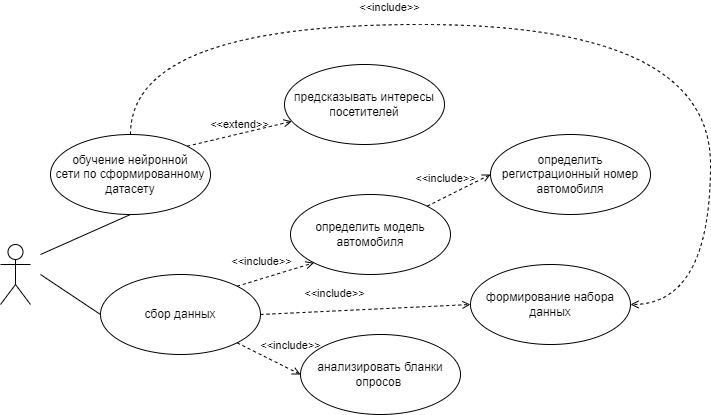
\includegraphics[width=0.7\textwidth]{diag-precedent1}
    \caption{Диаграмма вариантов использования}
    \label{f:diag-precedent1}
\end{figure}

\subsubsection{Основание для разработки}

Программа разрабатывается на основе учебного плана кафедры “Электронные вычислительные машины” по направлению 09.03.01.

\subsubsection{Цель и задача}

Название темы: «Разработка системы оценки и прогнозирования интересов клиентов автостоянки».

Объект - маркетинговое исследование для улучшения качества обслуживания клиентов.

% система оценки и прогнозирования интересов клиентов автостоянки.

Предмет - прогнозирования интересов клиентов автостоянки.

Целью дипломного проекта является помощь маркетологам в понимании предпочтений владельцев автомобилей через автоматизированный сбор и анализ данных, что позволит разрабатывать более точные и персонализированные маркетинговые стратегии. 

Задачи:
\begin{itemize}
    \item автоматизация процесса сбора данных;
    \item распознавание интересов посетителей парковки;
    \item прогнозирование интересов посетителей парковки;
\end{itemize}
% автоматизация процесса сбора данных об интересах посетителей парковки и их прогнозирования.

Результат - разработанная программная система для сбора информации о интересах клиентов и их прогнозироваения. 

\subsubsection{Наименование и область применения}

Наименование разрабатываемого программного обеспечения: система оценки и прогнозирования интересов клиентов автостоянки. 

Область применения: прогнозирование интересов посетителей парковки для улучшения сервиса.


\subsubsection{Требования к функциональности}

Программа должна обеспечивать возможность выполнения следующих функций:

\begin{itemize}
	\item определять регистрационный номер автомобиля;
	\item определять модель автомобиля
	\item анализировать бланки опросов определенного формата;
	\item формирование набора данных в файл типа CSV;
	\item обучение нейронной сети по сформированному датасету;
	\item предсказывать интересы посетителей с использование обученной модели.
\end{itemize}


\subsubsection{Требования к нейронной сети}

Нейронная сеть должна быть реализована на базе языка программирования Python с использованием библиотеки Tensorflow, Keras.


\subsubsection{Требования к бланку}

Бланк должен содержать вопросы и варианты ответа на вопросы (ДА/НЕТ), а также поле для ввода возраста. Пример представлен на рисунке~\ref{f:blank}.

\begin{figure}[ht]
	\centering
	\vspace{\toppaddingoffigure}
	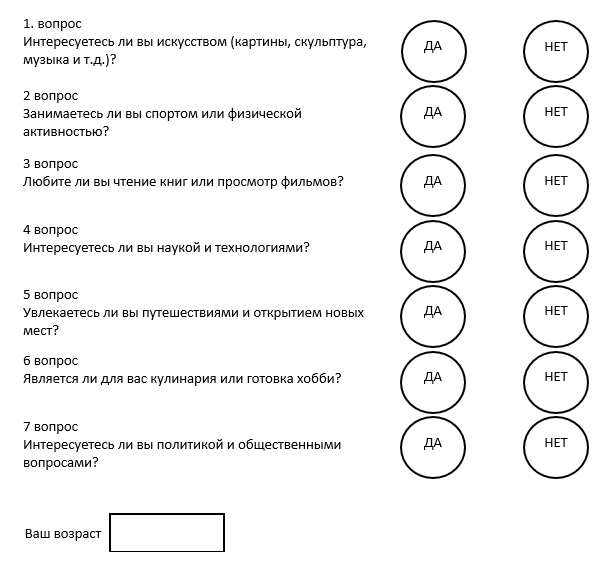
\includegraphics[width=0.7\textwidth]{blank}
	\caption{Бланк опроса}
	\label{f:blank}
\end{figure}



\subsubsection{Требования к программной документации}

Состав программной документации должен включать в себя: 

\begin{itemize}
	\item техническое задание; 
	\item пояснительная записка, содержащая описание разработки;
	\item руководство пользователя.
\end{itemize}

Разрабатываемые программные модули должны быть самодокументированы, т.е. тексты программ должны содержать все необходимые комментарии.

\subsubsection{Технико-экономические характеристики}

Реализованное программное обеспечение использует бесплатную модель распространения и разрабатывается с помощью бесплатных решений.


\section*{Выводы}

В данном разделе был проведен анализ предметной области, подчеркнута актуальность разработки модуля для анализа интересов посетителей парковки. 
Система представляет собой средство сбора информации об интересах и более точного и автоматизированного предсказания интересов посетителей парковки. Определение интересов клиентов позволяет оптимизировать уровень сервиса, а также разрабатывать персонализированные предложения для посетителей.
Также составлено техническое задание. Были составлены требования к разрабатываемой системе, а также определены основные функции. 



